%
%  Teori.tex
%  Part of VertEgg documentation
%

\chapter{Theory of Vertical Egg Distributions}

\section{The Equations}\label{sec:equations}


Neglecting horizontal processes, the evolution of the vertical
distribution
of a class of fish eggs is governed by a simple \emph{conservation}
principle\index{conservation principle}

\begin{equation}\label{eq:consprin}
\begin{split}
  \text{The change}\ & \text{in the number of eggs between two depth levels} \\
  & = \text{the number of eggs entering at the lower level} \\
  & - \text{the number of eggs leaving at the upper level} \\
  & + \text{the number of eggs spawned} \\
  & - \text{the number of eggs that hatched or died}
\end{split}
\end{equation}

To put this in a more mathematical formulation, let the variable
$z$ denote depth and $t$ time. The $z$-axis is chosen to point
\emph{up}, that is $z = 0$ at the surface and negative values are
used in the water column. This choice is opposite from
\cite{sund83,sund91} and \cite{west89}. The present choice is
motivated by the most
common axis-convention in 3D hydrodynamic ocean modelling.

To make the theory more convenient mathematically, a
\emphi{continuum} approach is used, where the eggs are
replaced by a continuous egg \emphi{concentration}.  Let $\phi =
\phi(z,t)$ denote this egg concentration at depth $z$ and time
$t$. Let $F = F(z,t)$ be the upwards egg \emphi{flux}, i.e.\ the net
number of eggs passing upwards per time unit at depth $z$ and time
$t$. Similarly, let $Q = Q(z,t)$ denote the \emphi{source term}, the
number of eggs spawned minus the numbers that hatched or died per
depth and time unit at depth $z$ and time $t$.  The source term can
also be used to take care of other processes, such as loss of eggs by
horizontal advection.

The conservation principle \ref{eq:consprin} can then be formulated
in \emphi{integral form}
\begin{equation}\label{eq:intlaw}
\int_{z_1}^{z_2} \!\phi(z,t_2)\,dz - \int_{z_1}^{z_2}\!\phi(z,t_1)\,dz
   = \int_{t_1}^{t_2} \!F(z_1,t)\,dt
   - \int_{t_1}^{t_2} \!F(z_2,t)\,dt
   + \int_{t_1}^{t_2}\!\int_{z_1}^{z_2} \!Q(z,t)\,dzdt
\end{equation}
Mathematically this can be reformulated in mixed form, differential in time
and integral in space
\begin{equation}\label{eq:diffintlaw}
  \pddt \left( \int_{z_1}^{z_2} \!\phi(z,t)\,dz \right) =
  F({z_1},t) - F({z_2},t) + \int_{z_1}^{z_2}\!Q(z,t)\,dz
  \quad \mbox{for} \ -H \le {z_1} < {z_2} \le 0 .
\end{equation}
or in pure \emph{differential} form\index{differential form}
\begin{equation}\label{eq:difflaw}
  \Pd{\phi}{t} =  - \Pd{F}{z} + Q
\end{equation}

The flux is decomposed in two parts, the \emphi{convective flux} and the
\emphi{diffusive flux}.  The convection is due to the terminal buoyant
velocity $w = w(z,t)$ of the egg which is computed by the density
difference from the surroundings  and the egg size as described in section
\ref{sec:velocity}. The formulation is simply,
\begin{equation}\label{eq:convflux}
  \Fconv = w \phi .
\end{equation}
The diffusion is caused by turbulent mixing and is modelled by
Fick's law\index{Fick's law} using the vertical eddy diffusion
\index{eddy diffusion} $K = K(z,t)$,
\begin{equation}\label{eq:fick}
  \Fdiff = - K \frac{\partial \phi}{\partial z} .
\end{equation}

Often the source term $Q$ can be separated in a
\emph{spawning}\index{spawning term} or \emph{production}
term\index{production term} independent of the egg concentration
\begin{equation}\label{eq:spawn}
  \Qspawn = P
\end{equation}
and a \emph{mortality}\index{mortality term} or \emph{loss}
term\index{loss term} depending on the concentration
\begin{equation}\label{eq:loss}
  \Qloss = - \alpha \phi
\end{equation}
Using this the differential conservation law (\ref{eq:difflaw})
becomes
\bel{eq:difflawfull}
\Pd{\phi}{t} =  - \pddz (w \phi) + \pddz (K \Pd{\phi}{z}) + P - \alpha \phi
\end{equation}
This parabolic partial differential equations is
called the \emph{convection-diffusion}\index{convection-diffusion equation}
or \emph{transport} equation\index{transport equation}.

The boundary conditions\index{boundary conditions} are simply no flux
across the surface and bottom,
\bel{eq:boundcond}
  F(0,t) = F(-H,t) = 0,
\end{equation}
and the initial condition is given by
\bel{eq:initcond}
  \phi(z,0) = \phi_0(z),  \quad -H \le z \le 0.
\end{equation}

\section{Solutions of the equations}

Under simplified circumstances the equations in section~\ref{sec:equations}
can be solved analytically. This section examines some of these solutions.

\subsection{Vertical integrated equation}\label{sec:vertint}

Let $\Phi$ denote the total concentration, $\Phi = \Vint \phi dz$.
Take the vertical integral of equation~(\ref{eq:difflawfull}) and
use the boundary conditions (\ref{eq:boundcond}) gives
\be
\Od{\Phi}{t} = P^{tot} - \Vint \!\alpha \phi \, dz
\end{equation}
where $P^{tot} = \Vint P dz$ is the total spawning contribution.
Without any source terms the total concentration $\Phi$ is constant.
To reach a steady state solution with spawning, the loss term $\alpha$
must be nonzero.


If $\alpha$ is a positive
constant, the solution to the equation above is
\be
  \Phi(t) = \e^{-\alpha t} \Phi(0)
         + (1 - \e^{-\alpha t})  \frac{P^{tot}}{\alpha}
\end{equation}
with steady state solution $\Phi = P^{tot}/\alpha$.
If $\alpha = 0$ the solution is simply
\be
  \Phi(t) = \Phi(0) + t P^{tot} .
\end{equation}


\subsection{Stationary solution}\index{stationary solution}

A stationary solution solves the conservation law
\pref{eq:difflaw} without the time derivative
\begin{equation}\label{eq:stateq}
  \Od{F}{z} = Q
\end{equation}
with boundary conditions $F(0) = F(-H) = 0$ given by \pref{eq:boundcond}.
The condition for the existence of this solution is that the total
source term vanishes,
\begin{equation}
  Q^{tot} = \Vint \!Q \, dz= 0
\end{equation}
the flux function is then given by integrating \pref{eq:stateq}
\begin{equation}
  F(z) = \int_{-H}^z \! Q(s) \, ds = - \int_z^0 \! Q(s) \, ds .
\end{equation}

Without source term the expression above reduces to $F = 0$, i.e.\ the
net flux is zero everywhere. This simply says that in a steady state
convection is balanced by diffusion
\bel{eq:sstate}
  w \phi - K \Pd{\phi}{z} = 0 .
\end{equation}
This is an ordinary differential equation for $\phi(z)$.
The boundary conditions \pref{eq:boundcond} does not contain more information.
A unique solution can nevertheless be singled out by the
integral condition
\begin{equation}\label{eq:intcond}
  \Vint \!\phi(z)\,dz = \Phi .
\end{equation}
In other words, among all the solutions of (\ref{eq:sstate})
choose the one with correct vertically integrated concentration.

To simplify the notation put $m = w / K$ and let $M(z) = - \int_z^0 m(s)
ds$. Then the stationary solution is
\begin{equation}\label{eq:sstatesol}
  \phi(z) = \frac{\Phi}{\int_{-H}^0 \e^{M(s)} ds} \e^{M(z)} .
\end{equation}

\subsubsection{Constant coefficients}

The case with constant coefficients was studied by Sundby
\shortcite{sund83}.  In this case $M(z) = m z$ and the solution is a
truncated exponential distribution,
\begin{equation}\label{eq:eggsact}
  \phi_m(z) = \Phi \frac{m}{1 - \e^{-mH}} \e^{mz} .
\end{equation}
In the toolbox, this solution is computed by the function \edbi{eggsact}.
This solution has the following symmetry between ascending and
descending velocity,
\begin{equation}\label{eq:symmetry}
  \phi_{-m}(z) = \phi_m(-H-z)
\end{equation}

With large depth and/or high ascending velocity  the
effect of the bottom may be neglected. In this case the distribution
is well approximated by an exponential distribution \index{exponential
distribution} with parameter $\lambda = 1 / m$, that is
\begin{equation}
  \phi_m(z) \approx \Phi m \e^{mz}, \quad \text{for $mH \gg 1$} .
\end{equation}


For positive values of $m$ the following series development from
\citep{sund83} is valid
\begin{equation}
  \phi_m(z) = \Phi m \e^{mz} \sum_{j = 0}^{\infty} \e^{-jmH}, \quad m > 0 .
\end{equation}
The zero-th term of this expansion is the exponential distribution above.
For negative values of $m$ the symmetry relation (\ref{eq:symmetry})
can be used,
\begin{equation}
  \phi_m(z) = - \Phi m \e^{mz} \sum_{j = 1}^{\infty} \e^{jmH}, \quad m < 0 .
\end{equation}

To compute the mean and variance of the distribution the constant
factor $\Phi$ can be dropped. The moment generating function is then
\begin{equation}\label{eq:momgen}
  \psi(t) = \int_{-H}^0 \frac{m}{1 - \e^{-mH}} \e^{(m+t)z} dz
          = \frac{m}{1 - \e^{-mH}} \frac{1 - \e^{-(m+t)H}}{m+t}.
\end{equation}
Differentiating $\psi$ gives the moments of the distribution.
The mean depth is given by
\begin{equation}\label{eq:eggsactmean}
  \mu = \psi'(0) = - \frac{1}{m} + \frac{H}{\e^{mH} - 1}
\end{equation}
The function $\mu = \mu(m)$ with $H = 100\m$ is plotted in
figure~\ref{fig:mdepth}.  The variance is
\begin{equation}\label{eq:eggsactvar}
       \psi''(0) - \mu^2
      = \frac{2 - \e^{-mH}(m^2 H^2 + 2 m H + 2)}{m^2 ( 1 - \e^{-mH})} - \mu^2
\end{equation}


\begin{figure}
\begin{center}
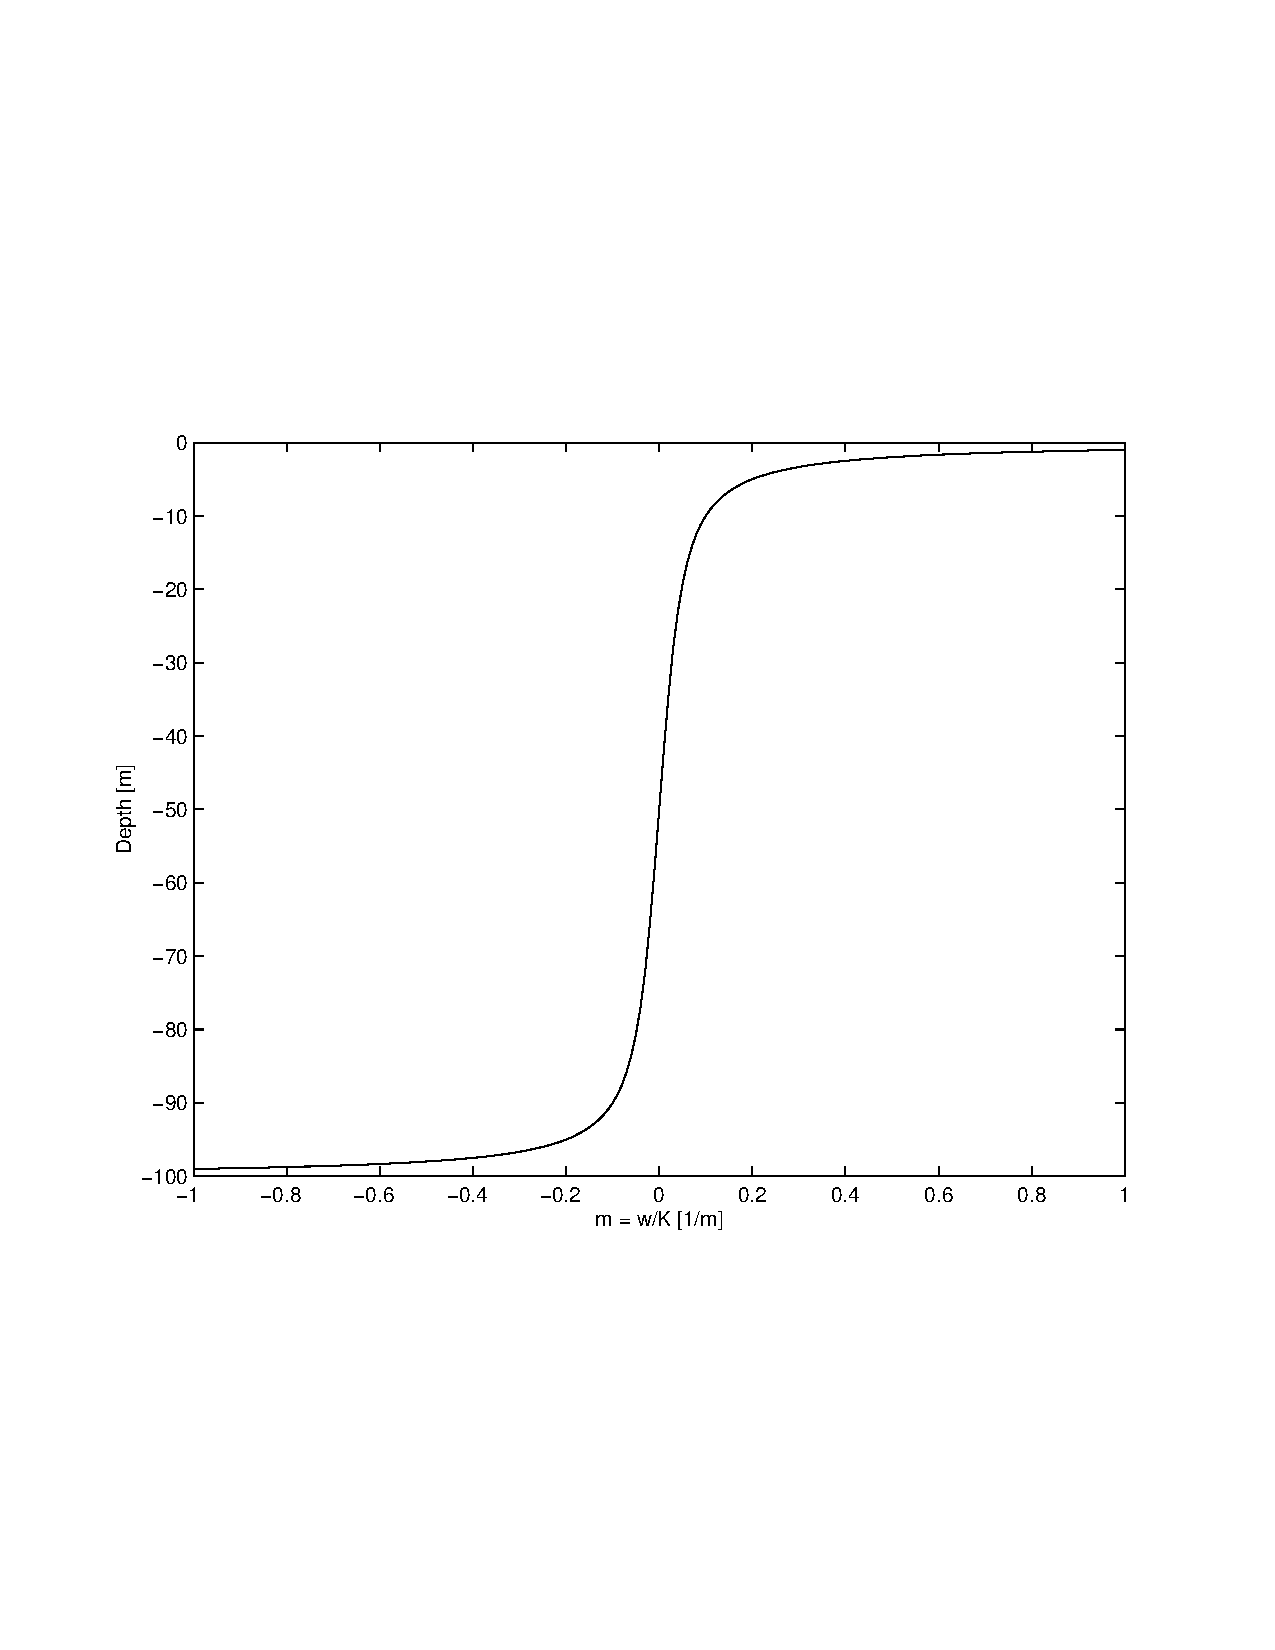
\includegraphics[height=6cm]{mdepth}
\end{center}
\caption{Mean depth $\mu$ as a function of $m$}\label{fig:mdepth}
\end{figure}

\subsubsection{Piecewise constant coefficients}

The solution (\ref{eq:eggsact}) can easily be extended to a piecewise
constant $m$.
Let $0 = z_0 > \cdots > z_m = -H$ be a partition of the water column
with $m(z) = m_i$ on the interval $I_i = (z_i, z_{i-1})$.
Then the stationary solution restricted to the interval $I_i$ is
given as
\begin{equation}\label{eq:pwconst}
  \phi(z) = C_i \e^{m_i z}, \quad \mbox{for} \ z_i < z < z_{i-1}
\end{equation}
The $C_i$-s are determined by continuity
of the solution
\begin{equation}
  C_i \e^{m_i z_i} = C_{i+1} \e^{m_{i+1} z_i}, \quad  i = 1, \ldots, m-1
\end{equation}
and the integral condition~(\ref{eq:intcond})
\begin{equation}
   \sum_{i = 1}^m C_i \int_{z_i}^{z_{i-1}} \e^{m_i z} dz
   = \sum_{i = 1}^m C_i \frac{\e^{m_i z_{i-1}} - \e^{m_i z_i}}{m_i}
   = \Phi .
\end{equation}
This method is used in the function \edbi{sstate} to approximate the
general steady state solution. More details of the implementation is
given in section~\ref{sec:statprob}.


\subsubsection{Linear coefficients}

In Sundby \shortcite{sund91} the solution is derived for $m$ linear.
Let $m$ be given as $m(z) = a (z-z_0)$. Then $M(z) =
\half a ((z - z_0)^2 - z_0^2)$. Taking the last term into the
constant $C$, the solution becomes
\begin{equation}
  \phi(z) = C \e^{\half a (z - z_0)^2} .
\end{equation}
Bathypelagic eggs are neutral buoyant at $z = z_0$, raising if deeper
and sinking if higher in the water column. In this case the coefficient
$a$ is negative and the concentration has a normal distribution about $z =
z_0$ with variance $\sigma^2 = {1 / |a|}$.

%In a sample of eggs the diameters and buoyancies differ from egg to egg.
%A more realistic model of the stationary situation will therefore be to
%use a distribution of the $m$-values. This task was studied by Sundby (1983).
%...


\subsubsection{Stationary solution with source terms}

With source terms, the steady state equation is
\begin{equation}\label{eq:srcsstate}
  0 = - \pddz (w \phi) + \pddz (K \Pd{\phi}{z}) + P - \alpha \phi .
\end{equation}
This is a general second order ordinary
differential equation. With constant coefficients the equation becomes
\begin{equation}\label{eq:srcsacteq}
  K \phi'' - w \phi' - \alpha \phi = - P
\end{equation}
and the no flux boundary conditions are
\begin{equation}
  K \phi' - w \phi, \quad z = 0, z = -H .
\end{equation}
The solution can be written
\bel{eq:srssact}
  \phi(z) = A \e^{az} - B \e^{-bz} + \frac{P}{\alpha}
\end{equation}
with
\begin{align}
  a & = \frac{1}{2K} ( \sqrt{w^2 + 4 \alpha K} + w ) \\
  b & = \frac{1}{2K} ( \sqrt{w^2 + 4 \alpha K} - w ) \\
  A & = \frac{w P}{\alpha b K} \frac{1-\e^{-b H}}{1-\e^{-(a+b)H}} \\
  B & = \frac{w P}{\alpha a K} \e^{-b H} \frac{1-\e^{-a H}}{1-\e^{-(a+b)H}} .
\end{align}

This function is computed in the toolbox by the function \edbi{srcsact}.
The signs are chosen such that positive velocity $w$ makes all terms
positive. For negative velocities a symmetry property
similar to equation~(\ref{eq:symmetry})
can be used, if
$\phi(z)$ is a solution to equation (\ref{eq:srcsacteq}) and boundary
conditions (\ref{eq:boundcond}) then $\phi(-H-z)$ is a solution the
same equation and boundary conditions with the opposite sign on $w$.
In other words,
\begin{equation}
  \phi_{-w}(z) = \phi_w(-H-z) .
\end{equation}


\section{The Terminal Egg Velocity}\label{sec:velocity}
\index{egg velocity}\index{terminal velocity}

An egg in sea water will reach its terminal velocity $w$, where the
buoyant forcing balances the frictional drag. This velocity is a
function of the difference $\Delta \rho = \rho - \rho_e$ between the
density of the water and the egg, the egg diameter $d$, the
acceleration $g$ due to gravity and the molecular
viscosity\index{molecular viscosity}. Here the \emph{dynamic}
molecular viscosity\index{dynamic viscosity} $\mu$ is used.

The situation is characterised by the non-dimensional \emphi{Reynolds
number},
\begin{equation}
  Re = \frac{\rho d w}{\mu}
\end{equation}
For low values, $Re < 0.5$, the terminal velocity is given by
\emphi{Stokes' formula}
\begin{equation}\label{eq:stokes}
  w = \frac{1}{18} \frac{g d^2 \Delta \rho}{\mu} .
\end{equation}
This formula was obtained by Stokes \shortcite{stok1851}. The
derivation of the formula is given in almost any textbook on
fluid dynamics, for instance \citep{yih77}.


Combining these equations, one obtains an expression for $D$, the maximum
diameter for which Stokes' velocity applies,
\begin{equation}
  D^3 = \frac{9 \mu^2}{\rho g \Delta \rho}
\end{equation}


In the intermediate region $0.5 < Re < 5$, Dallavalle (1948) gave an
empirical formula\index{Dallavalle's formula}
\begin{equation}\label{eq:dallavalle}
  w = K_I (d - \zeta D) \Delta \rho^{2/3} \mu^{-1/3}
\end{equation}
where $\zeta = 0.4$ for a sphere. The coefficient $K_I$ is determined
by the requirement that both formulas should give the same answer for
$Re = 0.5$ or equivalently $d = D$.
This gives
\begin{equation}
  K_I = \frac{5}{54} 9^{1/3} g^{2/3} \rho^{-1/3}
         = 0.0875 \text{kg}^{-1/3} \,
             \text{m}^{5/3} \text{s}^{-4/3} .
\end{equation}

The formulas above are implemented as the function \edbi{eggvel} in
the VertEgg toolbox. The buoyancy of a fish egg is often given as the
salinity $S_e$ where the egg is neutrally buoyant. The function
\edbi{eggvelst} computes the terminal velocity in this case.


To compute the egg velocity the density, $\rho$ of water is needed.
In the toolbox only density at surface pressure is presently
available.  This is computed by the function \edbi{dens0} by the
UNESCO formula \citep{UNES81}.  The function \edbi{sw\_dens} in the
SEAWATER toolbox\index{SEAWATER} \citep{morg94} has implemented the
full UNESCO equation of state.

The dynamic molecular
viscosity\index{viscosity!molecular}\index{viscosity!dynamic} $\mu$ of
sea water is tabulated in table \ref{tab:molvisc} taken from Sverdrup
\emph{et al.}
\shortcite{sver52}. The values decrease  with temperature and increase
slowly with salinity. The dependence on pressure is insignificant, and is
neglected here.

\begin{table}[h]
\begin{center}
\begin{tabular}{|c|c|c|c|c|c|c|c|}
\hline\hline
Salinity   & \multicolumn{7}{c|}{Temperature [\deg C]} \\
\cline{2-8}
[psu] & 0 & 5 & 10 & 15 & 20 & 25 & 30 \\
\hline
 0 & 1.79 &  1.52 & 1.31 & 1.14 & 1.01 & 0.89 & 0.80 \\
10 & 1.82 &  1.55 & 1.34 & 1.17 & 1.03 & 0.91 & 0.82 \\
20 & 1.85 &  1.58 & 1.36 & 1.19 & 1.05 & 0.93 & 0.84 \\
30 & 1.88 &  1.60 & 1.38 & 1.21 & 1.07 & 0.95 & 0.86 \\
35 & 1.89 &  1.61 & 1.39 & 1.22 & 1.09 & 0.96 & 0.87 \\
\hline
\end{tabular}
\end{center}
 \caption{Dynamic molecular viscosity of sea water
  with unit $10^{-3} \,\text{kgm}^{-1}\text{s}^{-1}$}
  \label{tab:molvisc}
\end{table}


Using linear least squares regression the table is approximated by the
following function where $T$ is the temperature in \deg C and $S$ is
the salinity in psu.
\begin{equation}\label{eq:molvisc}
  \mu = 10^{-3} \, (1.7915 - 0.0538 \, T + 0.007 \, T^2 - 0.0023 \, S )
            \:   \text{kgm}^{-1}\text{s}^{-1} ,
\end{equation}
This reproduces table \ref{tab:molvisc} with an absolute error less
than $2 \times 10^{-5}\, \text{kgm}^{-1}\text{s}^{-1}$ and a relative
error of 1.7 \%. This is good enough to compute egg velocities where
the uncertainty in the other variables are larger.  This formula is
implemented by the function
\edbi{molvisc} in the toolbox. Riley and Skirrow \shortcite{rile75}
give a more precise formula which requires more computational effort.
